\include{settings}

\begin{document}	% начало документа

% Титульная страница
\begin{titlepage}	% начало титульной страницы

	\begin{center}		% выравнивание по центру

		\large Санкт-Петербургский политехнический университет Петра Великого\\
		\large Институт компьютерных наук и технологий \\
		\large Высшая школа интеллектуальных систем и суперкомпьютерных технологий\\[6cm]
		% название института, затем отступ 6см
		
		\huge Низкоуровневое программирование\\[0.5cm] % название работы, затем отступ 0,5см
		\large Отчет по лабораторной работе №1\\[0.1cm]
		\large Машина Тьюринга-Поста\\[5cm]

	\end{center}


	\begin{flushright} % выравнивание по правому краю
		\begin{minipage}{0.25\textwidth} % врезка в половину ширины текста
			\begin{flushleft} % выровнять её содержимое по левому краю

				\large\textbf{Работу выполнил:}\\
				\large Аникин Д.А.\\
				\large {Группа:} 3530901/90004\\
				
				\large \textbf{Преподаватель:}\\
				\large Алексюк А.О.

			\end{flushleft}
		\end{minipage}
	\end{flushright}
	
	\vfill % заполнить всё доступное ниже пространство

	\begin{center}
	\large Санкт-Петербург\\
	\large \the\year % вывести дату
	\end{center} % закончить выравнивание по центру

\end{titlepage} % конец титульной страницы

\vfill % заполнить всё доступное ниже пространство


% Содержание
% Содержание
\renewcommand\contentsname{\centerline{Содержание}}
\setcounter{tocdepth}{1}
\tableofcontents
\newpage



\section{Цель работы}
Построить машину Тьюринга-Поста, вполняющую вычитание чисел в десятичном коде (уменьшаемое >= вычитаемому). Выполнить моделирование ее работы в одном из свободно доступных симуляторов. 

\section{Правила кодирования}

\subsection{Алфавит машины}
Алфавит машины состоит из следующих символов: ''-'' (разделение уменьшаемого и вычитаемого); Символы 1, 2, 3, 4,5, 6, 7, 8, 9,  используются для записи чисел в десятичном коде. Символы A, B, C, D, E, F, G, H, I, J являются вспомогательными - они не присутствуют на входной и выходных лентах.

\subsection{Кодирование входной ленты}
Перед запуском машины на входной ленте должны быть представлены уменьшаемое и вычитаемое (уменьшаемое >= вычитаемому). Числа длжны быть разделены символом ''-''. Головка машины указывает на последний символ представления вычитаемого.

\subsection{Кодирование выходной ленты}
Результатом работы машины при корректных входных данных является разность между введенными числами. Головка машины указывает на первый символ этого представления.

\section{Построение машины}
Для организации вычитания необходимо поочередно вычитать единицу из каждого разряда (заменить символ десятичной цифры n на n-1) вычитаемого и уменьшаемого, начиная с последнего. После того, как в разряде вычитаемого остается 0, он затирается, а соответствующая положению разряда вычитаемого цифра уменьшаемого маркируется специальным символом - буквой латинского алфавита (0 = A, 1 = B,..., 9 = J), чтобы игнорировать этот разряд в дальнейшем, так как процесс вычитания для него закончен. Альтернативный вариант - перемещать эти разряды в специальное место на ленте, отведенное для ответа, но он требует большее количество шагов и состояний. Процесс повторяется до тех пор, пока вычитаемое полностью не сотрется с ленты. Далее все маркированные цифры восстанавливаются до своего значения, машина завершает свою работу.

Машина начинает свою работу с состояния CHK0B0, проверяющее младший разряд вычитаемого на равенство нулю.
\begin{itemize}
\item 
Если младший разряд равен нулю, он затирается, производится переход в состояния MARKA0, производящее переход к разряду уменьшаемого. Затем происходит переход в состояние MARKA1, заменяющее цифру на букву, после чего осуществляется переход в состояние MVB0, возвращающее положение головки машины на место последнего оставшегося разряда, затем обратно в состояние CHK0B0.
\item
В противном случае переходим с состояние SUBB0, вычитающее единицу из разряда и переходящее затем в состояние MVA0 (перемещение к последнего разряду уменьшаемого). В состоянии MVA0 головка машины доходит до ''-'', происходит переход в MVA1, при котором головка движется влево, пропуская все маркированные разряды, пока не встретит первую цифру. Происходит переход в CHK0A0. 
\end{itemize}

Состояние CHK0A0, проверяет разряд уменьшаемого, по аналогии с CHK0B0, на равенство нулю.
\begin{itemize}
\item 
Если разряд равен нулю, значит необходимо сделать заём из старшего разряда. Из состояния CHK0A0 происходит переход в BORROW0. BORROW0 заменяет 0 на 9 и перемещает головку влево или, если нули закончились, переходит в SUBA0 для вычета единицы.
\item
Иначе переходим в SUBA0, вычетающее единицу из разряда уменьшаемого и переходящее в состояние MVB0, всё по аналогии с вычитаемым. Стоит отметить, что, если цифра в разряде равна единице, то происходит переход в SUBA1, которое проверяет, не является ли данный разряд старшим (не стоит ли перед ним пустой символ). Если нет, то происходит переход в SUBA3, заменяющее единицу на ноль. Если да - в состояние SUBA2, стирающее данный разряд.
\end{itemize}

Когда вычитаемое полностью стерлось, т.е в состоянии SUBB0 головка переходит к ''-'', начинается процесс восстановления уменьшаемого. Происхоит переход в RESTORE0, заменяющее буквенное представлени разрядов на численное и двигающее головку влево. При достижении пустого символа, что говорит о том, что все разряды восстановлены, происходит переход в завершающее состояние HALT. Машина останавливает свою работу.

\section{Результат построения}
Граф управляющего автомата построенной машины показан на Рис. 4.1. Итоговое количество состояний - 16.
\begin{figure}[H]
	\begin{center}
		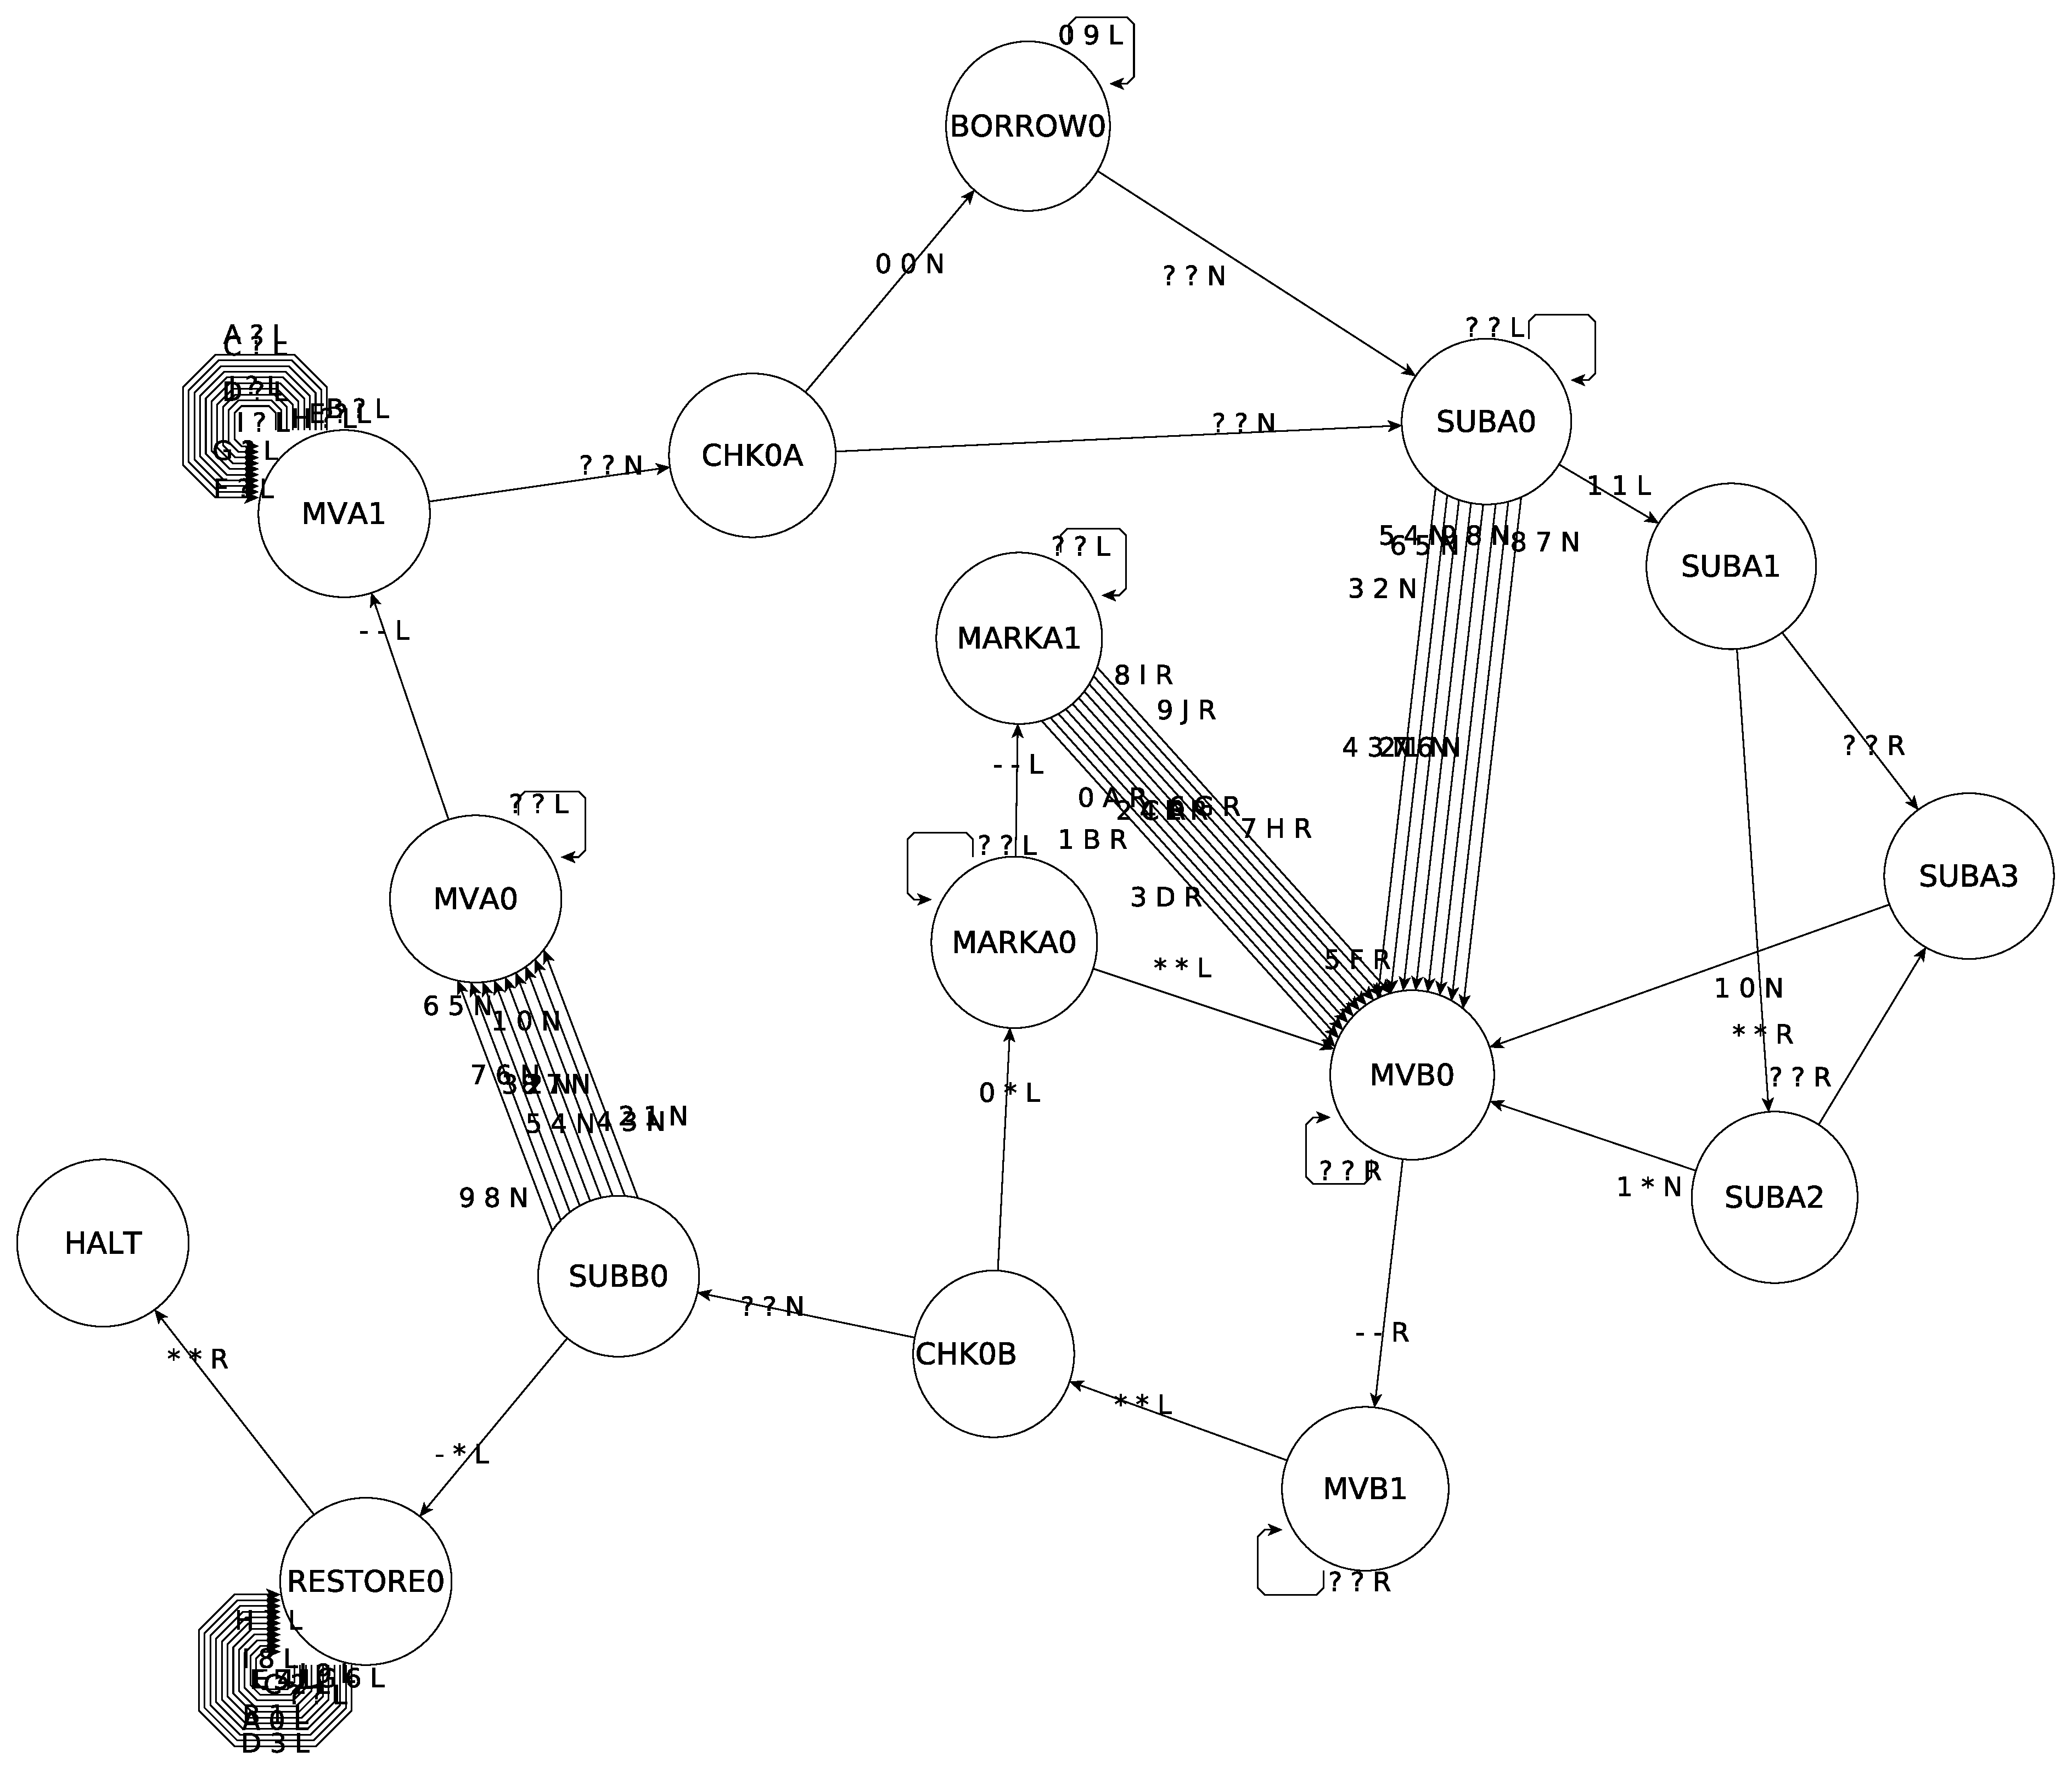
\includegraphics[scale=0.2]{graph}
		\caption{Граф переходов} 
		\label{pic:graph} % название для ссылок внутри кода
	\end{center}
\end{figure}

\section{Выводы}
В ходе работы была построена машина Тьюринга-Поста, выполняющее вычитание чисел в десятичном коде. В процессе работы постоянно происходит перемещение от разрядов уменьшаемого к вычитаемому и наоборот. Можно уменьшить количество выполняемых шагов и состояний, если построить многоленточную машину Тьюринга.

Данную машину можно доработать до вычитания и в случаях, когда уменьшаемое < вычитаемого. Для этого нужно в состоянии MVB0 проверить, не стоит ли пустой символ перед ''-''. Если да, то уменьшаемое полностью стерто, оставшийся результат является ответом, машина останавливается.
\end{document}
